\section{Инфраструктура проекта}

\subsection{Архитекрутра}
За основу берётся архитектурный паттерн \acrshort{mvc}. Он предполагает разделение данных приложения, пользовательского интерфейса и управляющей логики на три отдельных компонента: Модель, Представление и Контроллер – таким образом, что модификация каждого компонента может осуществляться независимо.

\begin{figure}[h]
    \begin{center}
        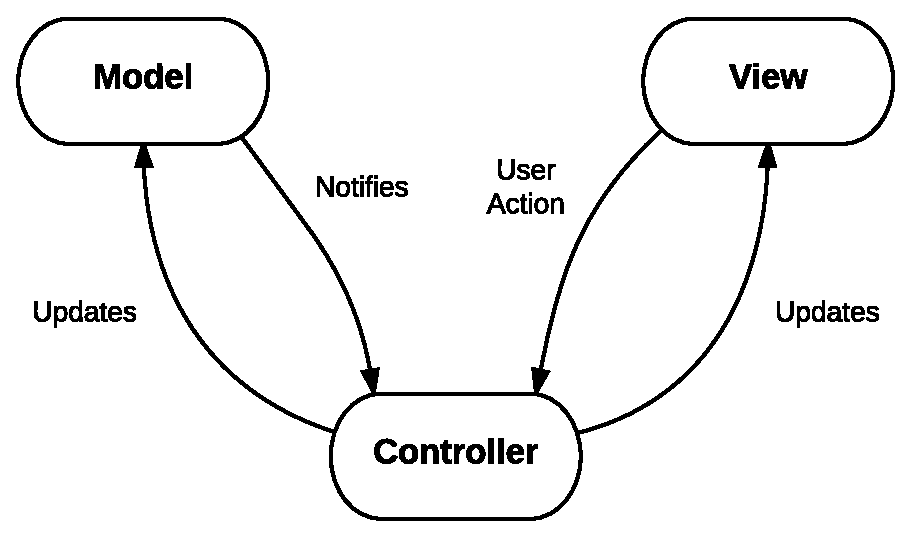
\includegraphics[scale=0.7]{images/MVC-basic.eps}
    \end{center}
    \caption{Визуализация архитектуры \acrshort{mvc}}
\end{figure}

\subsubsection{Связь логических компонетов и применяемых технологих}
\begin{itemize}
    \item Model --- \textcite{seqorm} для сервера и \textcite{redux} для клиента.
    \item View --- \textcite{react}
    \item Controller --- \textcite{express}
\end{itemize}

\subsection{Организация работы с Git}
\subsection{Сущности}

\subsection{Организация работы с \textcite{git}}
Для организации работы с системой контроля версий в проекте используется подход Git Workflow. Он нужен для согласованного и продуктивного выполнения работы.

\begin{figure}[h!]
    \begin{center}
        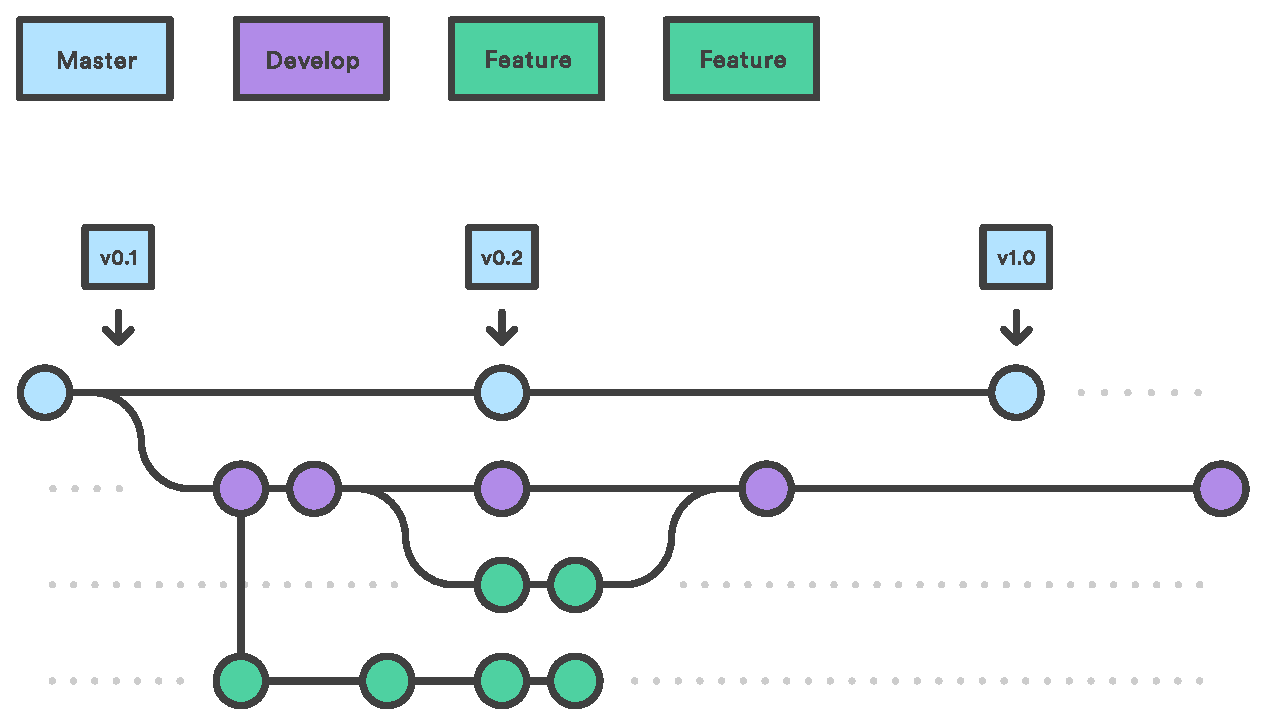
\includegraphics[scale=0.6]{images/git-workflow.eps}
    \end{center}
    \caption{Пример использования подхода Git Workflow}
\end{figure}

\clearpage